\documentclass{beamer}



% Language setting
% Replace `english' with e.g. `spanish' to change the document language
% \usepackage[english]{babel}

% Set page size and margins
% Replace `letterpaper' with `a4paper' for UK/EU standard size
%\usepackage[letterpaper,top=2cm,bottom=2cm,left=3cm,right=3cm,marginparwidth=1.75cm]{geometry}

% Useful packages
\usepackage{amsmath}
\usepackage{tikz}
\usetikzlibrary{trees}
\usetikzlibrary{positioning} 
\usetikzlibrary{arrows}
\usetikzlibrary{decorations.pathmorphing}
\usetikzlibrary{shapes.multipart}
\usetikzlibrary{shapes.geometric}
\usetikzlibrary{calc}
\usetikzlibrary{positioning} 
\usetikzlibrary{fit}
\usetikzlibrary{backgrounds}
\usetikzlibrary{automata}
\usepgflibrary{shapes.geometric}
\usetikzlibrary{shapes.geometric}
\usepackage{mathpartir}
\usepackage{listings}
\usepackage{proof}
\newtheorem{theorem}{Theorem}
\newtheorem{lemma}{Lemma}

\usepackage{graphicx}
%\usepackage[colorlinks=true, allcolors=blue]{hyperref}


\lstdefinelanguage{L4}
{morekeywords={
      assert 
    , class  
    , decl   
    , defn   
    , extends
    , lexicon
    , fact   
    , rule   
    , derivable
    , let   
    , in    
    , not   
    , forall
    , exists
    , if   
    , then 
    , else 
    , for  
    , true 
    , false
},    
sensitive=false,
morecomment=[l]{\#},
morestring=[b]",
}

\lstset{frame=tb,
  language=L4,
  aboveskip=3mm,
  belowskip=3mm,
  showstringspaces=false,
  columns=flexible,
  basicstyle={\footnotesize\ttfamily},
  numbers=none,
  numberstyle=\tiny\color{gray},
  keywordstyle=\color{blue},
  commentstyle=\color{green},
  stringstyle=\color{mauve},
  breaklines=true,
  breakatwhitespace=true,
  tabsize=2
}

%%% Local Variables: 
%%% mode: latex
%%% TeX-master: "main"
%%% End: 

% Theorems and definitions

% \newtheorem{definition}{Definition}
% \newtheorem{theorem}{Theorem}
% \newtheorem{lemma}{Lemma}
% \newtheorem{proposition}{Proposition}


% Definition of colors
\newcommand{\blue}[1]{{\color{blue}#1}}
\newcommand{\green}[1]{{\color{green}#1}}
\newcommand{\red}[1]{{\color{red}#1}}
\newcommand{\gray}[1]{{\color{gray}#1}}

% From MSCS file
\newcommand{\eg}{\textit{e.g.\ }}
\newcommand{\etal}{\textit{et al.\ }}
\newcommand{\etc}{\textit{etc}}
\newcommand{\ie}{\textit{i.e. }}
\newcommand{\viz}{\textit{viz.\ }}
\newcommand{\wrt}{\textit{w.r.t.\ }}
\newcommand{\lex}{\langle}
\newcommand{\rex}{\rangle}

% Own abbreviations
\newcommand{\secref}[1]{Section~\ref{#1}}
\newcommand{\secrefs}[1]{Sections~\ref{#1}}
\newcommand{\figref}[1]{Figure~\ref{#1}}
\newcommand{\figrefs}[1]{Figures~\ref{#1}}
\newcommand{\pgref}[1]{page~\pageref{#1}}
\newcommand{\theoremref}[1]{Theorem~\ref{#1}}
\newcommand{\theoremrefs}[1]{Theorems~\ref{#1}}
\newcommand{\lemmaref}[1]{Lemma~\ref{#1}}
\newcommand{\exampleref}[1]{Example~\ref{#1}}
\newcommand{\defref}[1]{Definition~\ref{#1}}

\newcommand{\figline}{\rule{\textwidth}{0.5pt}}


% Logique

\newcommand{\IMPL}[0]{\longrightarrow}
\newcommand{\IMPLL}[0]{\Longrightarrow} % another implication, to make
                                % a difference with reduction relations
\newcommand{\AND}[0]{\land}
\newcommand{\OR}[0]{\lor}
\newcommand{\NOT}[0]{\lnot}
\newcommand{\FALSE}[0]{\perp}
\newcommand{\TRUE}[0]{\top}
\newcommand{\IFF}[0]{\leftrightarrow}
\newcommand{\BIGAND}[1]{\bigwedge_{#1}}
\newcommand{\BIGOR}[1]{\bigvee_{#1}}
\newcommand{\BIGANDC}[2]{\bigwedge_{#1|#2}} % bigand with constraint
\newcommand{\BIGORC}[2]{\bigvee_{#1|#2}}    % bigor with constraint

\newcommand{\exgeq}[1]{\exists^{{\geq #1}}}
\newcommand{\exeq}[1]{\exists^{{= #1}}}
\newcommand{\exle}[1]{\exists^{{< #1}}}

% Remark macros for the authors

\newcommand{\remms}[2][]{\todo[color=green!40,#1]{MS: #2}}
\newcommand{\remre}[2][]{\todo[color=blue!40,#1]{RE: #2}}
\newcommand{\remjhb}[2][]{\todo[color=blue!20,#1]{JHB: #2}}


% Other

\newcommand{\smalltalcq}[0]{{\small small}-t{$\cal ALCQ$}}
\newcommand{\smalltalcqe}[0]{{\small small}-t{$\cal ALCQ$e}}
\newcommand{\trule}[0]{\xhookrightarrow}
\newcommand{\tableaurule}[1]{{\xhookrightarrow[]{#1}}}
\newcommand{\nodes}[1]{{\cal N}({#1})}
\newcommand{\trans}[1]{{\cal T}({#1})}
\newcommand{\transm}[1]{{\cal T'}({#1})}
\newcommand{\rconts}[1]{\llparenthesis #1 \rrparenthesis} %record contents
\newcommand{\rupd}[2]{{#1}\llparenthesis #2 \rrparenthesis} %record update

\newcommand{\eform}[0]{\mathit{eform}}
\newcommand{\form}[0]{\mathit{form}}
\newcommand{\free}[0]{\mathit{free}}
\newcommand{\exclprop}[0]{\stackrel{\times}{\longrightarrow}}

%%% Local Variables: 
%%% mode: latex
%%% TeX-master: "main"
%%% End: 


\title[Compliance through Model Checking]{Waicom~2022\\Compliance through Model Checking}

\author{Avishkar Mahajan \and \underline{Martin Strecker} \\\ Watt Seng Joe \and Meng Weng Wong}
\date{2022-12-14}

\institute{Singapore Management University / Toulouse University}

%======================================================================

\begin{document}


%======================================================================

\begin{frame}
  \titlepage
\end{frame}


%======================================================================
\section{CCLAW}


%-------------------------------------------------------------
\begin{frame}[fragile]\frametitle{Singapore's Centre for Computational Law}

  \blue{General outline:}
  \begin{quote}
    CCLAW's flagship programme researches and develops open source
    technologies for ‘smart’ contracts and ‘smart’ statutes, starting with the
    design and implementation of a \blue{domain-specific programming language} (DSL)
    that allows for laws, rules and agreements to be expressed in code. \\
    (From \red{\bf \url{https://cclaw.smu.edu.sg}})
  \end{quote}

  \blue{Relevant for this talk:}
  \begin{itemize}
  \item (Processing contracts)
  \item Reasoning \emph{with} contracts
  \item Reasoning \emph{about} contracts
  \end{itemize}
  \dots{} Facets of \red{compliance}
  
\end{frame}

%-------------------------------------------------------------
\begin{frame}[fragile]\frametitle{The L4 DSL and Ecosystem}

\begin{center}
\begin{tikzpicture}
[auto,
decision/.style={diamond, draw=blue, thick, fill=blue!20,
  text width=4.5em, text badly centered,
  inner sep=1pt},
block/.style ={rectangle, draw=blue, thick, fill=blue!20,
  text width=5em, text centered, rounded corners,
  minimum height=4em},
blockwide/.style ={rectangle, draw=blue, thick, fill=blue!20,
  text width=7em, text centered, rounded corners,
  minimum height=2em},
redblock/.style ={rectangle, draw=red, thick, fill=red!20,
  text width=5em, text centered, rounded corners,
  minimum height=4em},
redblockwide/.style ={rectangle, draw=red, thick, fill=red!20,
  text width=7em, text centered, rounded corners,
  minimum height=2em},
blockverif/.style ={rectangle, draw=green, thick, fill=green!20,
  text width=5em, text centered, rounded corners,
  minimum height=4em},
blockunverif/.style ={rectangle, draw=red, thick, fill=red!20,
  text width=8em, text centered, rounded corners,
  minimum height=4em},
line/.style ={draw, thick, -latex'},
cloud/.style ={draw=orange, thick, ellipse,fill=orange!30,
  minimum height=2em},
every node/.style={node distance=5mm and 15mm}]

\node [block] (naturall4) {Natural L4}; 
\begin{onlyenv}<1,3>
\node [block, below=of naturall4] (nlp) {NLP};
\end{onlyenv}
\begin{onlyenv}<2>
\node [redblock, below=of naturall4] (nlp) {NLP};
\end{onlyenv}
\node [block, right=of naturall4] (corel4) {Core L4}; 
\node [blockwide, right=of corel4] (ruleeng) {Rule engines: Prolog, ASP}; 
\node [blockwide, above=of ruleeng] (procmod) {Processes: BPMN, DMN};
\node [blockwide, below=of ruleeng] (smt) {SMT solver}; 
\begin{onlyenv}<1,2>
\node [blockwide, below=of smt] (automata) {Automata};
\end{onlyenv}
\begin{onlyenv}<3>
\node [redblockwide, below=of smt] (automata) {Automata};
\end{onlyenv}

\begin{scope}[every path/.style=line]
\path (naturall4) -- (corel4);
\path (naturall4) -- (nlp);
\path (nlp) -- (corel4);
\path (corel4) -- (ruleeng);
\path (corel4) -- (procmod);
\path (corel4) -- (smt);
\path (corel4) -- (automata);

\end{scope}

\end{tikzpicture}
\end{center}

\begin{onlyenv}<2>
See talk: \red{Ranta, Listenmaa, Soh, Wong: 
\emph{An End-to-End Pipeline from Law Text to Logical Formulas}}, Thursday, session~8
\end{onlyenv}

\begin{onlyenv}<3>
This talk: Modeling with automata
\end{onlyenv}
\end{frame}

%-------------------------------------------------------------
\begin{frame}[fragile]\frametitle{Natural L4: Legal Spreadsheets}

  \begin{center}
    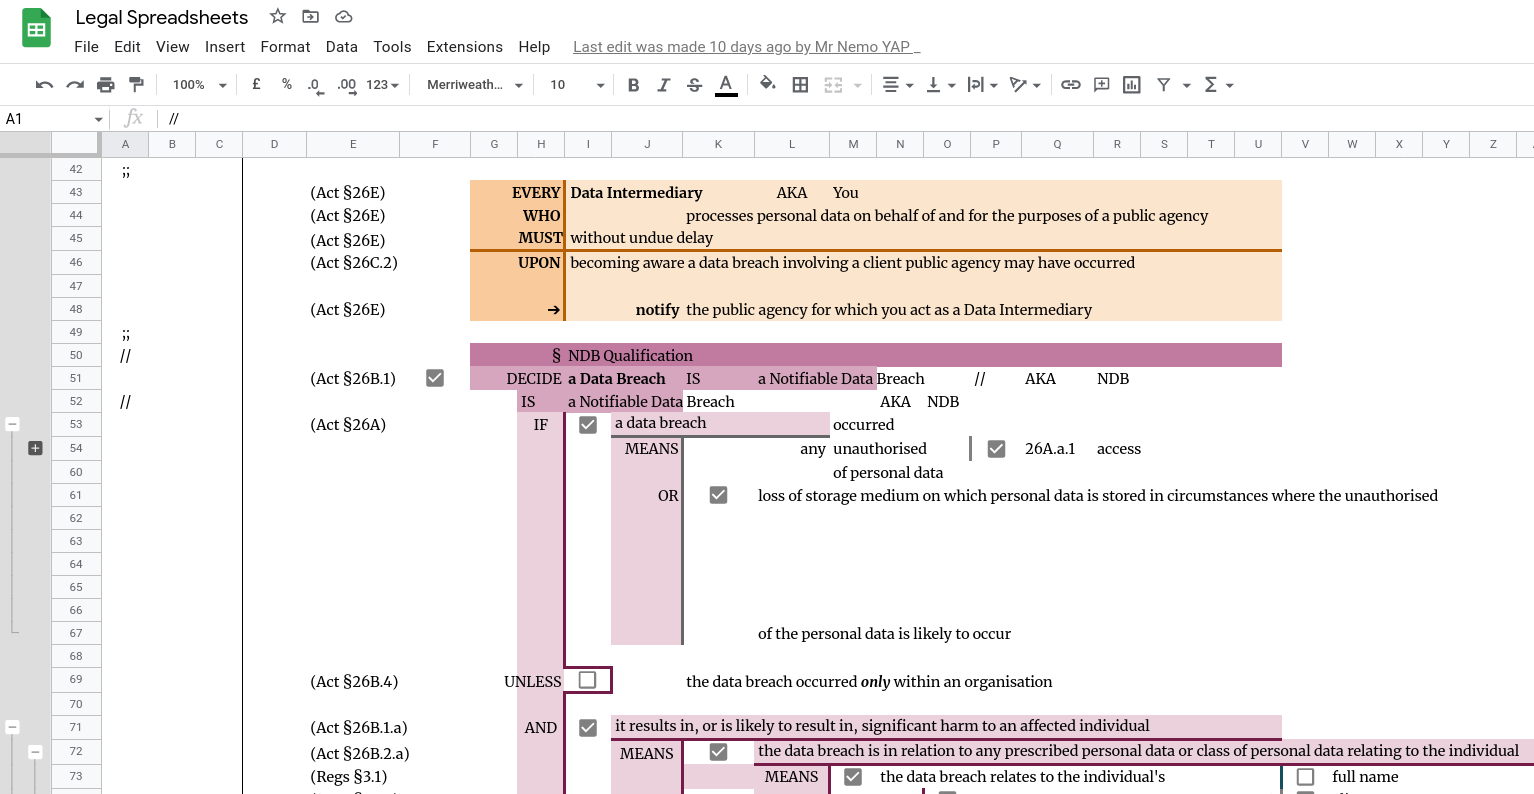
\includegraphics[scale=0.3]{Figures/legal_spreadsheets.png}
  \end{center}

\end{frame}


%-------------------------------------------------------------
\begin{frame}[fragile]\frametitle{Core L4: Intermediate DSL}

  \begin{center}
    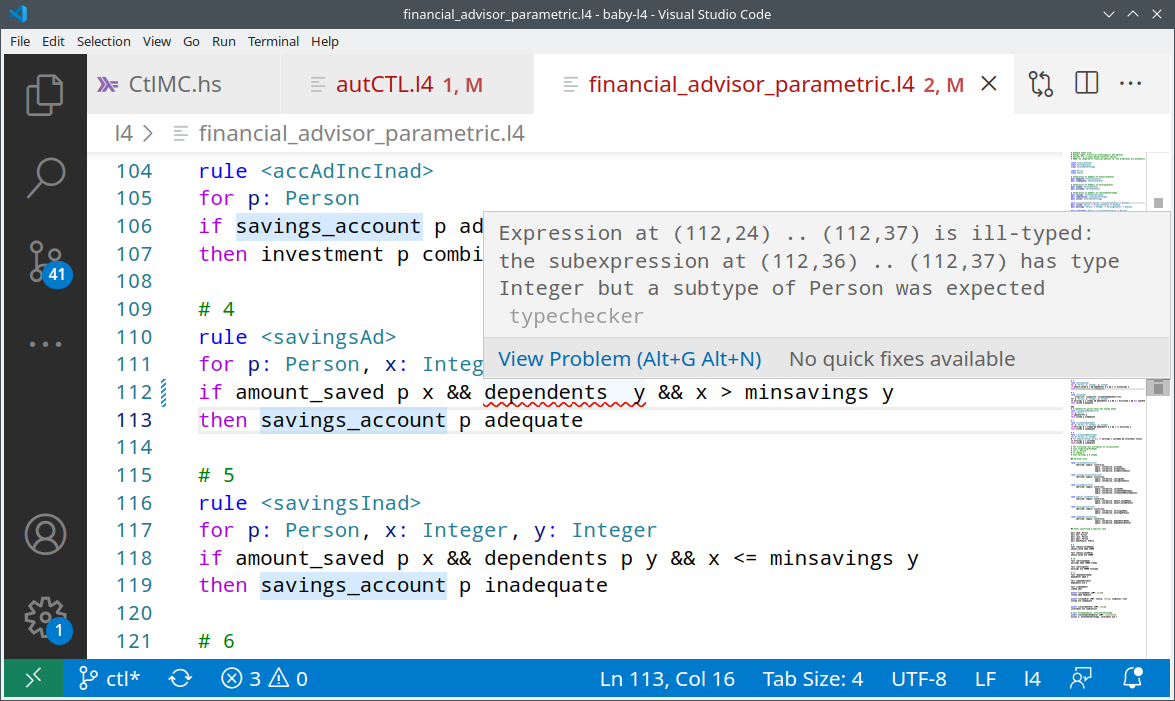
\includegraphics[scale=0.3]{Figures/corel4_typecheck.png}
  \end{center}
\end{frame}


%======================================================================
\section{Reasoning with and about Rules}




%======================================================================
\section{PDPA Case Study}



%======================================================================
\section{Future Work}



%-------------------------------------------------------------
\begin{frame}[fragile]\frametitle{What's the difference?}

  \blue{Reasoning \emph{with} rules:}
  \begin{itemize}
  \item Given:
    \begin{itemize}
    \item A set of rules  (\emph{e.g.: insurance contract})
    \item A specific scenario (\emph{e.g.: dammage / accident})
    \end{itemize}
  \item Sought:
    \begin{itemize}
    \item A judgement (\emph{who pays / how much?})
    \item Possibly with a justification (\emph{why?})
    \end{itemize}
  \end{itemize}

  \vspace{4mm}
  \blue{Reasoning \emph{about} rules:}
  \begin{itemize}
  \item Given:
    \begin{itemize}
    \item A set of rules  (\emph{e.g.: insurance contract})
    \item A notion of rule consistency
    \end{itemize}
  \item Sought:
    \begin{itemize}
    \item \emph{Either} an inconsistent scenario 
    \item \emph{or} a proof of consistency
    \end{itemize}
  \end{itemize}


\end{frame}

%-------------------------------------------------------------
\begin{frame}[fragile]\frametitle{Example: AXA insurance case study - \emph{Rules}}

  \dots{} about the coverage provided for the vehicle breakdown

  \blue{What is covered}
  \begin{itemize}
  \item If the vehicle breaks down more than one mile from your home, we will
    arrange and pay for a breakdown vehicle to come to the vehicle (for up to
    one hour) to try to get it working again.
    
  \item If the vehicle cannot be made safe to drive at the place you have
    broken down, we will arrange for the vehicle, the driver and passengers to
    be recovered to a repairer or a destination of your choice within 20 miles
    of where you have broken down.
  \end{itemize}
  
  \blue{What is not covered}
  \begin{itemize}
  \item A breakdown at or within one mile from your home.  
  \item Travel outside the UK.  
  \end{itemize}


\end{frame}

%-------------------------------------------------------------
\begin{frame}[fragile]\frametitle{Example: AXA insurance case study}

  \blue{Reasoning \emph{with} rules}
  
Is a cover provided for a mechanical breakdown in Swansea (that is 10 miles
away from home)?

\begin{lstlisting}
fact premiumPaid
fact currentSit mechanicalBrkd
fact situationInLocation mechanicalBrkd swansea
fact distance home swansea 10

assert <scen1_assert2> {SMT: valid} 
coverProvided mechanicalBrkd payBreakdownVehicle
\end{lstlisting}
\emph{Answer: Yes}

\end{frame}

%-------------------------------------------------------------
\begin{frame}[fragile]\frametitle{Example: AXA insurance case study}

  \blue{Reasoning \emph{about} rules}
  
  \begin{itemize}
  \item Is the rule set inconsistent?
  \item More precisely: Is there a situation such that the insurance has to
    pay and can refute payment?
  \end{itemize}
  
  \begin{lstlisting}
    for mySit: Situation, myCov: CoverageType
    assert <contradictoryCover> {SMT: consistent}
    coverProvided mySit myCov && myCov /= noCoverProvided &&
    coverProvided mySit noCoverProvided
  \end{lstlisting}
\vspace{-5mm}
  \emph{Answer:} Scenario:
  \begin{lstlisting}
    currentSit mechanicalBrkd
    coverProvided mechanicalBrkd noCoverProvided
    coverProvided mechanicalBrkd payBreakdownVehicle
    isBreakdownSituation mechanicalBrkd
    isIn home uk
    isIn dundalk abroad
    distance home dundalk d =  (15 <= d) && (d < 19)
  \end{lstlisting}
  
\end{frame}


%-------------------------------------------------------------
\begin{frame}[fragile]\frametitle{Evaluation}

  \blue{What's the interest?}
  \begin{itemize}
  \item Sanitize your rules before running them in production mode
  \item Similar to software verification before deployment
  \end{itemize}

  \vspace{4mm}
  \blue{Where are the difficulties?}
  \begin{itemize}
  \item \emph{Input:} Rules and \emph{lots} of everyday knowledge
    \begin{itemize}
    \item Geography
    \item Components of a car
    \item No breakdown in two different locations at the same time
    \end{itemize}
  \item \emph{Input:} Notion of consistency
  \item \emph{Output:} Comprehensible display of scenarios
  \end{itemize}

\end{frame}



%======================================================================
\section{Reasoning with and about Processes}


%-------------------------------------------------------------
\begin{frame}[fragile]\frametitle{Rules and Automata}

  An antagonistic view? \emph{No!}

\blue{Rules} for modelling time-independent situations

\blue{Automata} for modelling time-dependent processes
\begin{itemize}
\item prevalent in today's Business Process Management tools
\item but what about compliance?
\end{itemize}

\begin{columns}
  \column{.5\textwidth}
  \begin{center}
  BPM languages:

    \includegraphics[scale=0.2]{Figures/business_process.png}
    
    \tiny{(from  SAP BPM pages)}
  \end{center}
  \column{.5\textwidth}
  \begin{center}
    Uppaal \red{(live demo!)}
  
    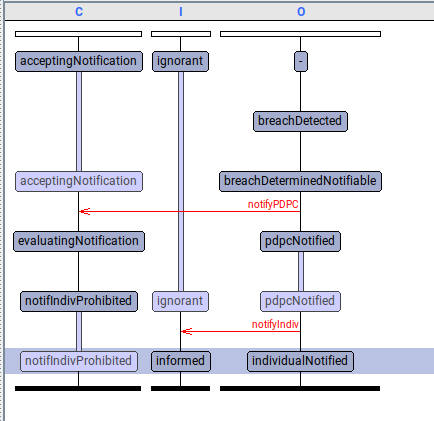
\includegraphics[scale=0.35]{Figures/uppaal_swimlane.png}
  \end{center}
\end{columns}

\end{frame}



%======================================================================
\section{Symbolic AI for the Law}


%-------------------------------------------------------------
\begin{frame}[fragile]\frametitle{Symbolic AI for the Law}

\blue{Main Framework: Logic Programming}
\begin{itemize}
\item Logic programming is a suitable paradigm for symbolic AI and thus can be used for computational law
\item Can naturally incorporate rule priorities/exceptions etc through defeasible reasoning
\end{itemize}

\vspace{4mm}
\blue{Logic Programming based Expert System}
\begin{itemize}
\item Generate questions automatically from a rule set and a query
\item Display justification graph for derived answer
\item Process is fully automated. When rule set changes so do the questions
\end{itemize}

\end{frame}



%-------------------------------------------------------------

\end{document}


%%% Local Variables: 
%%% mode: latex
%%% TeX-master: t
%%% coding: utf-8
%%% End: 
